\documentclass[tikz,border=10pt]{standalone}
\usepackage{tikz}
\usetikzlibrary{arrows.meta}
\begin{document}
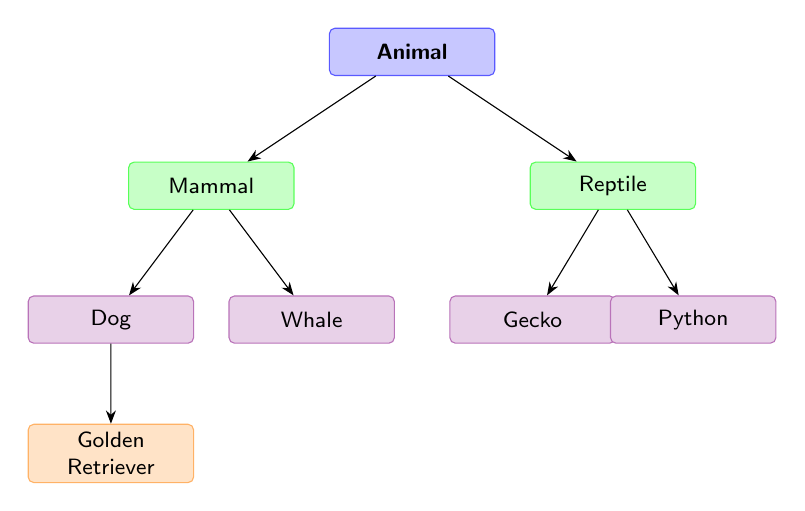
\begin{tikzpicture}[
  scale=0.85,
  every node/.style={rounded corners=2pt, font=\footnotesize\sffamily, align=center,
                     draw, minimum width=2.1cm, minimum height=0.6cm, inner sep=3pt},
  root/.style={fill=blue!22, draw=blue!65, font=\footnotesize\bfseries\sffamily},
  lvl1/.style={fill=green!22, draw=green!65},
  lvl2/.style={fill=violet!18, draw=violet!55},
  lvl3/.style={fill=orange!22, draw=orange!60},
  lbl/.style={draw=none, fill=none, font=\tiny\itshape, minimum width=0pt, minimum height=0pt,
              inner sep=1pt}
]
  \node[root] (animal) at (0,0) {Animal};
  \node[lvl1] (mammal) at (-3,-2) {Mammal};
  \node[lvl1] (reptile) at (3,-2) {Reptile};
  \node[lvl2] (dog) at (-4.5,-4) {Dog};
  \node[lvl2] (whale) at (-1.5,-4) {Whale};
  \node[lvl2] (gecko) at (1.8,-4) {Gecko};
  \node[lvl2] (python) at (4.2,-4) {Python};
  \node[lvl3] (goldenret) at (-4.5,-6) {Golden\\Retriever};
  \draw[->,>=Stealth] (animal) -- (mammal);
  \draw[->,>=Stealth] (animal) -- (reptile);
  \draw[->,>=Stealth] (mammal) -- (dog);
  \draw[->,>=Stealth] (mammal) -- (whale);
  \draw[->,>=Stealth] (reptile) -- (gecko);
  \draw[->,>=Stealth] (reptile) -- (python);
  \draw[->,>=Stealth] (dog) -- (goldenret);
\end{tikzpicture}
\end{document}
